\documentclass[border=3pt]{standalone}
\usepackage{palatino}
\usepackage[T1]{fontenc}
\usepackage[utf8]{inputenc}
\usepackage{amsmath,amssymb}
\usepackage{tikz}
\usetikzlibrary{arrows.meta,shapes,positioning,decorations.pathreplacing}
\usepackage{xcolor}

\definecolor{lrGray}{HTML}{6E6D66}
\definecolor{lrBlue}{HTML}{444D8A}
\definecolor{lrBlueDk}{HTML}{2E3566}
\definecolor{lrRasp}{HTML}{B0485F}
\definecolor{lrRaspDk}{HTML}{8F3A4D}
\definecolor{lrInk}{HTML}{33322F}
\definecolor{lrLabel}{HTML}{5C5B57}

\begin{document}
  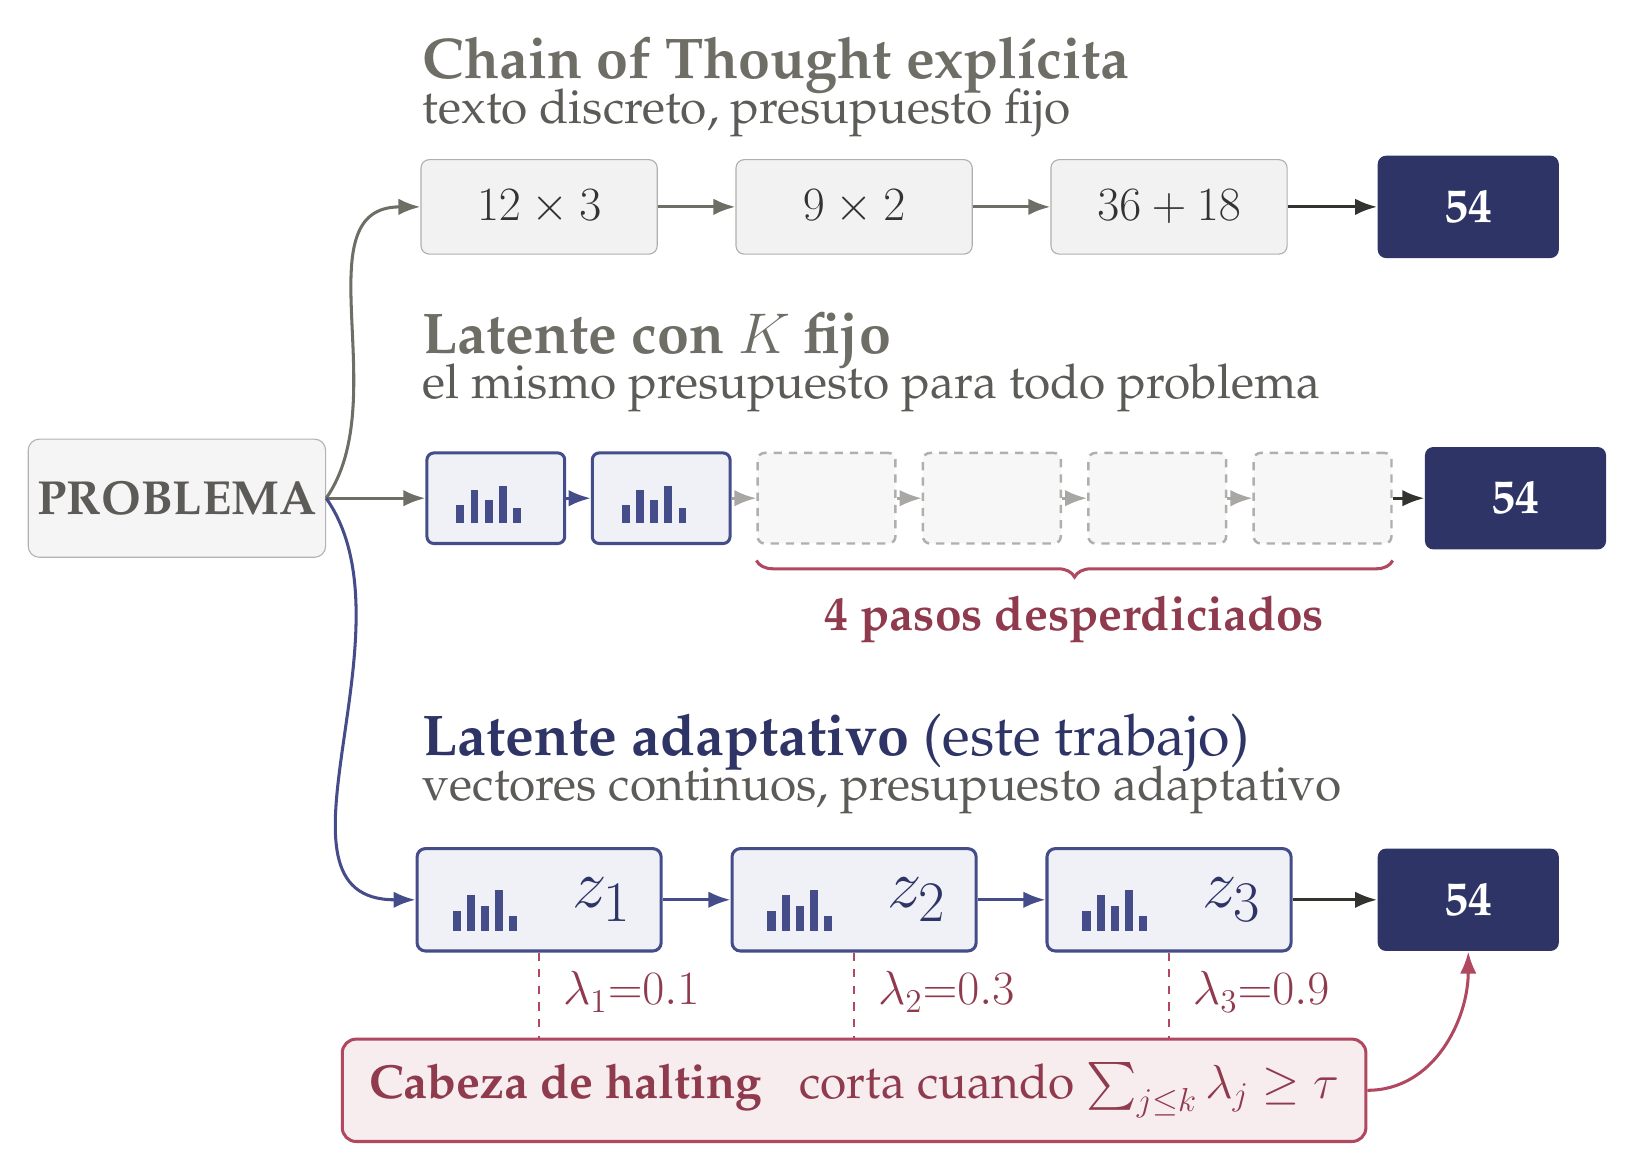
\begin{tikzpicture}[
      font=\rmfamily,
      >={Latex[length=2.8mm]},
      stepbox/.style={rounded corners=3pt, minimum width=3.0cm, minimum height=1.2cm,
                  inner sep=2pt, align=center,
                  draw=lrGray!55, fill=black!5, text=black!80, font=\LARGE},
      zb/.style={rounded corners=3pt, minimum width=3.1cm, minimum height=1.3cm,
                 align=center, inner sep=2pt,
                 draw=lrBlue, line width=1.1pt, fill=lrBlue!8},
      % carril de K fijo: cajas chicas, usadas vs. desperdiciadas
      zsmall/.style={rounded corners=2.5pt, minimum width=1.75cm, minimum height=1.15cm,
                 align=center, inner sep=1pt,
                 draw=lrBlue, line width=1.1pt, fill=lrBlue!8},
      zwaste/.style={rounded corners=2.5pt, minimum width=1.75cm, minimum height=1.15cm,
                 align=center, inner sep=1pt,
                 draw=lrGray!55, line width=0.9pt, dash pattern=on 3pt off 2.5pt,
                 fill=black!3},
      ans/.style={rounded corners=3pt, fill=lrBlueDk, text=white,
                  minimum width=2.3cm, minimum height=1.3cm, font=\LARGE\bfseries},
      title/.style={anchor=west, font=\huge\bfseries},
      sub/.style={anchor=west, font=\LARGE, text=lrLabel},
      lam/.style={anchor=north, font=\LARGE, text=lrRaspDk},
    ]

    % ---------- entrada compartida (izquierda, centrada sobre los tres carriles) ----------
    \node[rounded corners=4pt, draw=black!30, fill=black!4,
          minimum width=2.9cm, minimum height=1.5cm, font=\LARGE\bfseries,
          text=lrLabel] (prob) at (1.1,-2.15) {PROBLEMA};

    % ================= carril 1: CoT explícita =================
    \node[title, text=lrGray] at (4.1,3.35) {Chain of Thought explícita};
    \node[sub]                at (4.1,2.75) {texto discreto, presupuesto fijo};

    \node[stepbox] (e1) at (5.7,1.55)   {$12\times 3$};
    \node[stepbox] (e2) at (9.7,1.55)   {$9\times 2$};
    \node[stepbox] (e3) at (13.7,1.55)  {$36+18$};
    \node[ans]  (ea) at (17.5,1.55) {54};

    \draw[->,lrGray, line width=1.1pt] (e1)--(e2);
    \draw[->,lrGray, line width=1.1pt] (e2)--(e3);
    \draw[->,lrInk,  line width=1.1pt] (e3)--(ea);

    % ================= carril 2: latente con K fijo =================
    \node[title, text=lrGray] at (4.1,-0.15) {Latente con $K$ fijo};
    \node[sub]                at (4.1,-0.75) {el mismo presupuesto para todo problema};

    \node[zsmall] (f1) at (5.15,-2.15) {};
    \node[zsmall] (f2) at (7.25,-2.15) {};
    \node[zwaste] (f3) at (9.35,-2.15) {};
    \node[zwaste] (f4) at (11.45,-2.15) {};
    \node[zwaste] (f5) at (13.55,-2.15) {};
    \node[zwaste] (f6) at (15.65,-2.15) {};
    \node[ans]    (fa) at (18.1,-2.15) {54};

    % glifo de vector sólo en los pasos que realmente se usan
    \foreach \n in {f1,f2}{
      \foreach \dx/\h in {-5.0mm/2.4mm, -3.2mm/4.2mm, -1.4mm/3.0mm, 0.4mm/4.8mm, 2.2mm/1.9mm}
        \fill[lrBlue] ([xshift=\dx, yshift=-3.2mm]\n.center) rectangle ++(1.0mm,\h);
    }

    \draw[->,lrBlue, line width=1.1pt] (f1)--(f2);
    \draw[->,lrGray!60, line width=1.0pt] (f2)--(f3);
    \draw[->,lrGray!60, line width=1.0pt] (f3)--(f4);
    \draw[->,lrGray!60, line width=1.0pt] (f4)--(f5);
    \draw[->,lrGray!60, line width=1.0pt] (f5)--(f6);
    \draw[->,lrInk,  line width=1.1pt] (f6)--(fa);

    % llave: los pasos que sobran
    \draw[decorate, decoration={brace, amplitude=6pt, mirror}, lrRasp, line width=1.1pt]
      ([yshift=-2mm]f3.south west) -- ([yshift=-2mm]f6.south east)
      node[midway, below=9pt, font=\LARGE\bfseries, text=lrRaspDk]
      {4 pasos desperdiciados};

    % ================= carril 3: latente adaptativo =================
    \node[title, text=lrBlueDk] at (4.1,-5.25) {Latente adaptativo \textnormal{(este trabajo)}};
    \node[sub]                  at (4.1,-5.85) {vectores continuos, presupuesto adaptativo};

    \node[zb] (z1) at (5.7,-7.25)   {};
    \node[zb] (z2) at (9.7,-7.25)   {};
    \node[zb] (z3) at (13.7,-7.25)  {};
    \node[ans](za) at (17.5,-7.25) {54};

    \foreach \n/\lbl in {z1/1, z2/2, z3/3}{
      \node[text=lrBlueDk, font=\Huge\itshape] at ([xshift=8mm]\n.center) {$z_{\lbl}$};
      \foreach \dx/\h in {-11mm/2.6mm, -9.2mm/4.6mm, -7.4mm/3.2mm, -5.6mm/5.2mm, -3.8mm/2.0mm}
        \fill[lrBlue] ([xshift=\dx, yshift=-4mm]\n.center) rectangle ++(1.05mm,\h);
    }

    \draw[->,lrBlue, line width=1.1pt] (z1)--(z2);
    \draw[->,lrBlue, line width=1.1pt] (z2)--(z3);
    \draw[->,lrInk,  line width=1.1pt] (z3)--(za);

    % ---------- cabeza de halting ----------
    \node[rounded corners=5pt, draw=lrRasp, line width=1.1pt, fill=lrRasp!10,
          anchor=north, minimum width=13cm, minimum height=1.3cm, inner sep=8pt,
          text=lrRaspDk, font=\LARGE] (halt) at (9.7,-9.0)
      {{\bfseries Cabeza de halting} \; corta cuando $\sum_{j\le k}\lambda_j \ge \tau$};

    \foreach \n/\lam in {z1/{\lambda_1{=}0.1}, z2/{\lambda_2{=}0.3}, z3/{\lambda_3{=}0.9}}{
      \draw[lrRasp, dashed, line width=0.9pt] (\n.south) -- (\n.south|-halt.north);
      \node[lam, anchor=west] at ([xshift=1.8mm, yshift=-5mm]\n.south) {$\lam$};
    }
    \draw[->,lrRasp, line width=1.1pt] (halt.east) to[out=0,in=-90] (za.south);

    % ---------- ramas: entrada -> los tres carriles ----------
    \draw[->,lrGray, line width=1.1pt] (prob.east) to[out=55, in=180] (e1.west);
    \draw[->,lrGray, line width=1.1pt] (prob.east) to[out=0,  in=180] (f1.west);
    \draw[->,lrBlue, line width=1.1pt] (prob.east) to[out=-55,in=180] (z1.west);

  \end{tikzpicture}
\end{document}
